\originalsection{实际第二次考试: Exam 2}
本节依据 MIT 8.03 Fall 2016 实际 Exam 2 原卷整理, 不属于 Practice Exam. 原卷共13页, 第1页为说明, 第2--7页为公式表, 第8--12页为四道题, 第13页为 OCW 版权说明. 四题总分100分. 请在答题册内作答, 试卷上作答不评分; 闭卷, 禁止电子设备, 手机、BlackBerry、Blueberry、Raspberry Pi、平板和电脑等须关机. 现有材料没有与本实际试卷配套的官方解答; 以下全部为\textbf{AI 独立解答}, 不借用练习卷答案充作官方答案. 本节不照抄公式表中的排印错误.

\begin{exercise}\label{exam:actual2.1}
原题 Problem 1 (30 pts). 回答下列短题. 原卷提示: 若某短题耗时很长, 可能未找对方向.
\begin{enumerate}[label=\Alph*.]
\item (6分) 一列行进平面电磁波射向理想导体; 导体内电荷可自由运动且无能量耗散. 电磁波电场在导体\textbf{表面而非内部}的边界条件是什么?
\item (6分) 载频为 $f$ 的 AM 广播台近期音质评价较差. 为改善信号的时间分辨率, 你建议台长增大还是减小发射带宽 $\Delta f$? 说明理由.
\item (6分) 房间尺寸为 $L\times L\times16L$, 空气中声速为 $v$. 室内空气简正振荡的最低角频率是多少?
\item (6分) 长度 $2L$ 的有质量弦, 两端固定在 $x=-L,L$, 张力 $T$, 线密度 $\rho_L$. $t=0$ 的形状如下, 随后小心从静止释放, 即 $\dot\psi(x,0)=0$. 在无色散弦上, 最早经过多久恢复初始形状? \textbf{不要实际作 Fourier 分解}, 但须解释. 原图的正凸起为居中平台上叠加圆滑小凸顶, 其尺寸未标数值; 重绘只保留该形状及端点、原点与基线, 不把示意长度当数据.
\begin{center}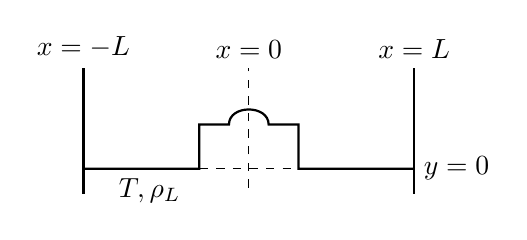
\begin{tikzpicture}[x=2.1cm,y=.8cm]
\draw[thick] (-1,-.4)--(-1,1.6);\draw[thick] (1,-.4)--(1,1.6);
\draw[dashed] (-1,0)--(1,0) node[right]{$y=0$};\draw[dashed] (0,-.3)--(0,1.6);
\draw[thick] (-1,0)--(-.30,0)--(-.30,.7)--(-.12,.7)
 .. controls (-.12,1.02) and (.12,1.02) .. (.12,.7)
 --(.30,.7)--(.30,0)--(1,0);
\node[above] at (-1,1.6){$x=-L$};\node[above] at (0,1.6){$x=0$};\node[above] at (1,1.6){$x=L$};
\node[below] at (-.6,0){$T,\rho_L$};
\end{tikzpicture}\end{center}
\item (6分) 光从真空 $n_1=1$ 先进入折射率 $n_2$ 的透明板, 入射角 $\alpha=60^\circ$; 穿过后再穿过 $n_3$ 的透明板, 最后进入第四介质 $n_4$, 与法线夹角 $\beta=45^\circ$. 原图三界面水平且互相平行, 两已知角均从竖直法线量起. 求 $n_4$. 示意图不提供板内角的数值.
\begin{center}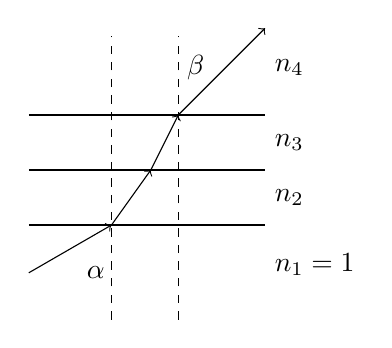
\begin{tikzpicture}[x=1cm,y=1cm]
\foreach \y in {0,.7,1.4}{\draw[thick] (-1.5,\y)--(1.5,\y);}
\draw[dashed] (-.45,-1.2)--(-.45,2.4);\draw[dashed] (.4,-1.2)--(.4,2.4);
\draw[->] (-1.5,-.6062178)--(-.45,0);\draw[->] (-.45,0)--(.05,.7);
\draw[->] (.05,.7)--(.4,1.4);\draw[->] (.4,1.4)--(1.5,2.5);
\node[right] at (1.5,-.5){$n_1=1$};\node[right] at (1.5,.35){$n_2$};
\node[right] at (1.5,1.05){$n_3$};\node[right] at (1.5,2){$n_4$};
\node at (-.65,-.6){$\alpha$};\node at (.62,2){$\beta$};
\end{tikzpicture}\end{center}
\end{enumerate}
\end{exercise}
\begin{solution}
\textbf{AI 独立解答.}
(A) 理想导体表面的\textbf{总电场切向分量}为零:
\[
\hat{\mathbf n}\times\mathbf E_{\rm total}=0,\qquad
\mathbf E_{i,\parallel}+\mathbf E_{r,\parallel}=0.
\]
这里是入射与反射场相加后的边界条件, 不要求入射波单独为零. 法向分量一般不为零; 真空侧满足 $\epsilon_0E_n=\sigma_s$, 可以由表面电荷支撑. 只有在正入射等使全部波电场均为切向的特殊情形, 表面总电场才整体为零. 理想导体不吸收功率, 不表示没有反射.

(B) 建议\textbf{增大}带宽. 变化更快的音频包含更高频率分量, 调幅后在载频 $f$ 两边产生相应边带. 更宽的带宽可容纳这些边带, 使较短时间尺度的变化得以保留. 典型时间尺度与带宽满足 $\Delta t\sim1/\Delta f$, 具体常数取决于带宽和脉冲宽度的定义. 这是带宽与时间分辨率的关系, 并不是只提高载频就自动改善音质.

(C) 令压强扰动为 $p$. 对房间的理想刚壁, 法向空气速度为零. 由 $\rho_0\partial_t\mathbf u=-\nabla p$ 得到振动压强的 Neumann 条件 $\partial_np=0$, 不能套用四边固定膜的 Dirichlet 条件. 取长边为 $z$ 轴, 空间模为
\[
p_{rst}\ \propto\ \cos\frac{r\pi x}{L}\cos\frac{s\pi y}{L}\cos\frac{t\pi z}{16L},
\quad r,s,t=0,1,2,\ldots,
\]
\[
\omega_{rst}=\frac{\pi v}{L}\sqrt{r^2+s^2+\frac{t^2}{16^2}}.
\]
$(0,0,0)$ 是空间常量零频静态压强变化, 不属于非零频率的声振荡. 排除它后, 最小取 $(r,s,t)=(0,0,1)$, 故
\[
\boxed{\omega_{\min}=\frac{\pi v}{16L}}.
\]
该模沿长边只有半个空间波长, 两短方向均匀, 因此长边而不是三边平方和决定最低频率.

(D) 设弦速 $v_s=\sqrt{T/\rho_L}$, 将坐标平移为 $s=x+L\in[0,2L]$, 初形记为 $F_0(s)$. 从静止释放的两个行波各为初形的一半, 以 $\pm v_s$ 传播. 固定端反射使位移反号. 把 $F_0$ 关于 $s=0$ 作奇延拓, 再作 $4L$ 周期延拓, 得 $F(s)$; 关于 $s=2L$ 也为奇对称. d'Alembert 公式为
\[
\psi(s,t)=\frac12[F(s-v_st)+F(s+v_st)].
\]
它直接满足两端固定和初速度为零, 没有作 Fourier 分解. 每个行波传播 $4L$ 后通过两次固定端反射, 回到原位置和原符号, 所以 $t=4L/v_s$ 必定恢复原形.

还须证明这不是一个晚于最早恢复的周期. 本题初形只有一个与零基线隔开的正凸起, 其奇延拓在一个 $4L$ 周期内恰有一个正凸起和一个负凸起. 因而 $F$ 的最小正空间周期为 $4L$: 小于 $4L$ 的平移不能把唯一正凸起的支撑区间保持不变. 这个结论不要求左右轮廓完全对称.

若某时刻 $t>0$ 恢复原形, 令 $h=v_st$, $G_\pm(s)=F(s\pm h)$. 原区间上的恢复由奇对称性和周期性扩展为整周期上 $(G_-+G_+)/2=F$. 移位不改变整周期的 $L^2$ 范数, 所以
\[
\left\|\frac{G_-+G_+}{2}\right\|^2
=\|F\|^2-\frac14\|G_--G_+\|^2.
\]
左侧等于 $\|F\|^2$, 故 $G_-=G_+$, 又因其平均为 $F$, 两者都等于 $F$. 因而 $h$ 必须是 $F$ 的空间周期, 最小为 $4L$. 这也适用于图中理想化折线或阶跃初形, 不须假定其斜率具有有限能量. 最早恢复时间因此是
\[
\boxed{t_{\rm first}=4L\sqrt{\rho_L/T}}.
\]
经过 $2L/v_s$ 时为反号后的左右镜像形状, 并非原来的正凸起. 某些特殊简正模或重复子结构可有更短恢复时间, 但图示单一正凸起不属于那类初态.

(E) 三个界面法线相同, 每次 Snell 定律保持同一个切向波数, 即
\[
n_1\sin\alpha=n_2\sin r_2=n_3\sin r_3=n_4\sin\beta.
\]
因此 $n_4=\sin60^\circ/\sin45^\circ=\sqrt{3/2}\simeq1.2247$. 中间层使射线位置横向偏移, 不改变最终切向波数. 这一消去依赖原图界面平行, 不能无条件用于转角不相同的串联界面.
\end{solution}

\begin{exercise}\label{exam:actual2.2}
原题 Problem 2 (17 pts). 等离子体的一维小电荷密度偏离 $\rho(x,t)$ 满足
\[
a^2\frac{\partial^2\rho}{\partial x^2}-\Omega_p^2\rho=\frac{\partial^2\rho}{\partial t^2},
\]
$\Omega_p$ 是常数等离子体频率参数, $a>0$ 是方程中的速度参数.
\begin{enumerate}[label=\alph*.]
\item (3分) 写一列沿 $-\hat{\mathbf x}$ 的简谐行波解, 波数大小 $k$, 角频率 $\omega$, 振幅 $A$, 且 $\rho(0,0)=0$.
\item (7分) 求色散关系 $\omega(k)$, 画其随 $k$ 的曲线. 哪些角频率的简谐行波能在等离子体存在?
\item (4分) 求群速度. 是否为色散介质?
\item (3分) 大波数极限的相速度是多少?
\end{enumerate}
\end{exercise}
\begin{solution}
\textbf{AI 独立解答.}
(a) 以 $k>0,\omega>0$ 表示大小, 可取
\[
\rho(x,t)=A\sin(kx+\omega t).
\]
等相位点满足 $x=-\omega t/k+\text{常量}$, 因而向负 $x$ 传播, 且原点初值为零. 整体负号亦允许.
(b) 对该波 $\rho_{xx}=-k^2\rho$, $\rho_{tt}=-\omega^2\rho$, 代回得到
\[
\boxed{\omega(k)=\sqrt{\Omega_p^2+a^2k^2}}.
\]
图以 $K=ak/\Omega_p$, $W=\omega/\Omega_p$ 为无量纲轴, 取 $\Omega_p>0$. 实行波要求 $\omega>\Omega_p$, 截止极限 $\omega=\Omega_p$ 对应 $k=0$, 只是空间均匀振荡而不是有非零波数的行进波. $0<\omega<\Omega_p$ 没有实波数的体内行波; 若由边界激励, 只能产生相应的空间倏逝场. 曲线关于带符号的 $k=0$ 对称.
\begin{center}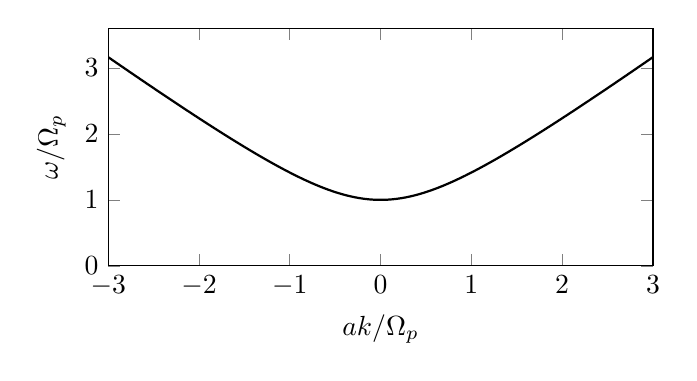
\begin{tikzpicture}
\begin{axis}[width=8.5cm,height=4.6cm,xmin=-3,xmax=3,ymin=0,ymax=3.6,xlabel={$ak/\Omega_p$},ylabel={$\omega/\Omega_p$},xtick={-3,-2,-1,0,1,2,3},ytick={0,1,2,3},samples=120]
\addplot[thick,domain=-3:3] {sqrt(1+x*x)};
\end{axis}\end{tikzpicture}\end{center}
(c) 对带符号波矢 $q$, $v_g=\dd\omega/\dd q=a^2q/\omega$. 对(a)向左的波, $q=-k$, 故群速度向左, 其大小为 $a^2k/\sqrt{\Omega_p^2+a^2k^2}$. 它随波数改变, 所以 $\Omega_p\ne0$ 时为色散介质. 当 $k\to0$, 群速趋零; 当 $k\to\infty$, 群速大小趋 $a$. 若参数恰为 $\Omega_p=0$, 则退化为普通无色散波动方程.
(d) 相速度大小为 $v_p=\omega/k=\sqrt{a^2+\Omega_p^2/k^2}$, 因而大波数极限为 $a$, 向左传播时带符号相速度为 $-a$. 相速度趋于的参数 $a$ 不应误认为光速 $c$; 该方程没有给出二者相等的条件.
\end{solution}

\begin{exercise}\label{exam:actual2.3}
原题 Problem 3 (23 pts). 真空中的均匀平面电磁波以光速 $c$ 传播, 电场为
\[
\mathbf E(\mathbf r,t)=E_0(3\hat{\mathbf x}+a\hat{\mathbf y})\cos(\omega t-4x+3y),
\]
其中 $a$ 是常数, 这是三维空间中的问题; 相位坐标系数取与 $x,y$ 的长度单位相容的逆长度单位.
\begin{enumerate}[label=\alph*.]
\item (4分) 用单位向量表示传播方向.
\item (6分) 用给定数值求角频率 $\omega$ 和波长.
\item (4分) 求 $a$.
\item (6分) 求相伴磁场 $\mathbf B$.
\item (3分) 求定向能流密度, 即单位面积能量传输率.
\end{enumerate}
\end{exercise}
\begin{solution}
\textbf{AI 独立解答.}
(a) 相位写为 $\omega t-\mathbf k\cdot\mathbf r$, 因而 $\mathbf k=4\hat{\mathbf x}-3\hat{\mathbf y}$, $|\mathbf k|=5$. 传播单位向量是
$\hat{\mathbf k}=(4\hat{\mathbf x}-3\hat{\mathbf y})/5$, 没有 $z$ 分量.
(b) 真空色散关系 $\omega=c|\mathbf k|$ 给 $\omega=5c$, $\lambda=2\pi/5$. 若原相位中的坐标按米计, 就是 $k=5\,\mathrm{m^{-1}}$, $\omega\simeq1.50\times10^9\,\mathrm{s^{-1}}$, $\lambda\simeq1.25664\,\mathrm m$.
(c) 横向性 $\mathbf k\cdot\mathbf E=0$ 要求 $12-3a=0$, 所以 $a=4$. 也可计算 $\nabla\cdot\mathbf E=E_0(12-3a)\sin(\omega t-4x+3y)$ 并令它恒为零. 电场真实振幅为 $5E_0$, 不是 $E_0$.
(d) 令 $\Phi=\omega t-4x+3y$. 真空磁场为
\[
\mathbf B=\frac1c\hat{\mathbf k}\times\mathbf E
=\frac{5E_0}{c}\hat{\mathbf z}\cos\Phi.
\]
叉乘系数为 $(4\times4+3\times3)/5=5$, 与 $|B|=|E|/c$ 相符. 传播方向在 $xy$ 平面不代表磁场也在该平面内.
(e) 瞬时 Poynting 向量是
\[
\mathbf S=\frac1{\mu_0}\mathbf E\times\mathbf B
=\frac{5E_0^2}{\mu_0c}(4\hat{\mathbf x}-3\hat{\mathbf y})\cos^2\Phi
=25\epsilon_0cE_0^2\hat{\mathbf k}\cos^2\Phi.
\]
周期平均定向能流密度为
\[
\boxed{\langle\mathbf S\rangle=\frac{25}{2}\epsilon_0cE_0^2\hat{\mathbf k}}.
\]
因此垂直传播方向的面上平均强度是 $25\epsilon_0cE_0^2/2$. 任意面法线 $\hat{\mathbf n}$ 上的通量为 $\langle\mathbf S\rangle\cdot\hat{\mathbf n}$.
\end{solution}

\begin{exercise}\label{exam:actual2.4}
原题 Problem 4 (30 pts). 长 $L$ 的有质量弦张力为 $T$, 线密度为 $\rho_L$, 只可沿 $\hat{\mathbf y}$ 上下运动. 左端 $x=0$ 固定于墙, 右端 $x=L$ 接在无质量圆环上; 圆环沿竖直杆无摩擦自由移动. 忽略重力, 全弦采用小角近似. 初形如图, 右侧宽 $2L/7$ 的部分高度为 $H$, 其余为零, $t=0$ 从静止释放. 初形在理想阶跃处按左右极限解释.
\[
f(x)=\psi(x,0)=\begin{cases}0,&0\le x<5L/7,\\H,&5L/7<x\le L,\end{cases}
\qquad \psi_t(x,0)=0.
\]
\begin{center}\begin{tikzpicture}[x=6cm,y=.9cm]
\draw[thick] (0,-.5)--(0,1.6);\draw[gray] (1,-.5)--(1,1.6);
\draw[dashed] (0,0)--(1,0);\draw[thick] (0,0)--(.7142857,0)--(.7142857,1)--(1,1);
\draw[thick] (1,1) ellipse (.022 and .08);
\draw[<->] (.7142857,1.4)--(1,1.4) node[midway,above]{$2L/7$};
\draw[<->] (1.1,0)--(1.1,1) node[midway,right]{$H$};
\node[below] at (0,-.5){$x=0$};\node[below] at (1,-.5){$x=L$};
\end{tikzpicture}\end{center}
\begin{enumerate}[label=\alph*.]
\item (8分) 用位移 $\psi(x,t)$ 写 $x=0,L$ 的边界条件.
\item (6分) 画三个最低简正模的形状, 不论它们是否被此初态激发, 并给其角频率.
\item (10分) 根据初形, 用 $n,H$ 求第 $n$ 个简正模的振幅.
\item (6分) 哪些模不被激发? 用 $n$ 表示.
\end{enumerate}
\end{exercise}
\begin{solution}
\textbf{AI 独立解答.}
(a) 固定左端给 $\psi(0,t)=0$. 右端环可上下动, 杆不提供竖直方向的约束力, 环又无质量且无重力, 所以弦张力的竖直分量必须为零. 小斜率下 $T\psi_x(L,t)=0$, 即
\[
\boxed{\psi(0,t)=0,\qquad\psi_x(L,t)=0}.
\]
自由环不是固定端, 也不是给定高度为 $H$ 的驱动端; $H$ 只是初始高度.
(b) 记 $v_s=\sqrt{T/\rho_L}$. 波动方程与两边界给
\[
k_n=\frac{(2n-1)\pi}{2L},\quad X_n(x)=\sin(k_nx),\quad
\omega_n=v_sk_n,\qquad n=1,2,3,\ldots.
\]
前三角频率是 $\pi v_s/(2L),3\pi v_s/(2L),5\pi v_s/(2L)$. 各模左端节点、右端零斜率的腹. 下图横轴 $x/L$, 纵轴为分别归一化的模幅度; 图外说明实线、虚线、点线分别表示 $n=1,2,3$, 不把峰幅当作此初态的实际振幅.
\begin{center}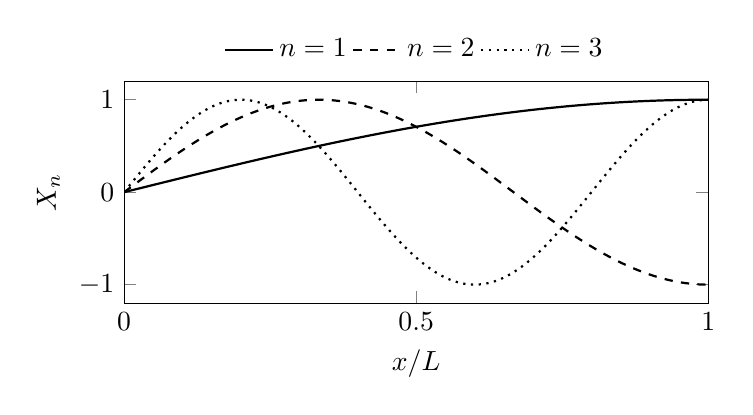
\begin{tikzpicture}
\begin{axis}[width=9cm,height=4.4cm,xmin=0,xmax=1,ymin=-1.2,ymax=1.2,xlabel={$x/L$},ylabel={$X_n$},samples=130,xtick={0,.5,1},ytick={-1,0,1},legend style={at={(.5,1.04)},anchor=south,legend columns=3,draw=none}]
\addplot[thick,domain=0:1] {sin(90*x)};\addlegendentry{$n=1$}
\addplot[thick,dashed,domain=0:1] {sin(270*x)};\addlegendentry{$n=2$}
\addplot[thick,dotted,domain=0:1] {sin(450*x)};\addlegendentry{$n=3$}
\end{axis}\end{tikzpicture}\end{center}
(c) 从静止释放使每个模只有余弦时间项,
\[
\psi(x,t)=\sum_{n=1}^{\infty}A_n\sin(k_nx)\cos(\omega_nt).
\]
这些空间模的正交归一为 $\int_0^L\sin(k_nx)\sin(k_mx)\dd x=(L/2)\delta_{nm}$. 因而
\[
\begin{aligned}
A_n&=\frac2L\int_0^Lf(x)\sin(k_nx)\dd x
=\frac{2H}{Lk_n}\left[\cos\frac{5k_nL}{7}-\cos(k_nL)\right]\\
&=\boxed{\frac{4H}{(2n-1)\pi}\cos\frac{5(2n-1)\pi}{14}}.
\end{aligned}
\]
利用 $\cos(k_nL)=0$ 可知振幅是有正负的模系数; 若称振幅为非负大小, 则用 $|A_n|$ 并把符号吸收进相位. 阶跃点处级数取值为 $H/2$, 不影响积分系数. 原题同时给阶跃示意与小角模型, 阶跃只应看作理想初形或很陡过渡的极限, 不将其解释为处处有限小斜率的实际弦形.
(d) 对 $H\ne0$, 未激发模的条件为
\[
\cos\frac{5(2n-1)\pi}{14}=0
\quad\Longleftrightarrow\quad
5(2n-1)=7(2j+1).
\]
因5与7互素, $2n-1$ 必须是7的奇数倍, 即 $2n-1=7(2\ell+1)$, $\ell=0,1,2,\ldots$. 反代确给余弦的奇数半周期零点. 所以
\[
\boxed{n=7\ell+4,\qquad \ell=0,1,2,\ldots}
\]
不被激发, 即 $n=4,11,18,\ldots$. 若改用零起始编号 $n'=n-1$, 同一集合为 $n'=7\ell+3$; 此处全程采用从1开始的原稿内部约定. 若 $H=0$, 初态为零, 全部模都不激发.
\end{solution}
